\section{Additional Related Work on Data-Centric Approach}\label{add:sec:related}
\paragraph{Data Augmentation}
Data augmentation creates new examples with preserved labels but uses no unlabeled data~\citep{shorten2019survey,kashefi2020quantifying,balestriero2022effects}. Examples of heuristic data augmentation techniques include flipping, distorting, and rotating images~\citep{shorten2019survey}, using lexical substitution, inserting words, and shuffling sentences in texts~\citep{kashefi2020quantifying}, and deleting nodes and dropping edges in graphs~\citep{zhao2021data,zhao2022graph}. While human knowledge can be used to improve data diversity and reduce over-fitting in heuristic methods, it is difficult to use a single heuristic method to preserve the different labels for different tasks~\citep{balestriero2022effects, cubuk2019autoaugment}. So, automated augmentation~\citep{cubuk2019autoaugment} learned from data to search for the best policy to combine a bunch of predefined heuristic augmentations. Generation models~\citep{antoniou2017data,bowles2018gan,han2022g} create in-class examples. Other learning ideas such as \textsc{FATTEN}~\citep{liu2018feature} and \textsc{GREA}~\citep{liu2022graph} learned to split the latent space for data augmentation. However, learning and augmenting from insufficient labels at the same time may limit the diversity of new examples and cause over-fitting. \method leverages unlabeled data to avoid them.

\paragraph{Relationship between Data-Centric Approaches} 
\begin{wrapfigure}{r}{5.5cm}
\caption{Qualitative relationship of graphs from different data-centric approach on the task relatedness and contained knowledge.}\label{fig: info relationship}
\resizebox{.8\linewidth}{!}{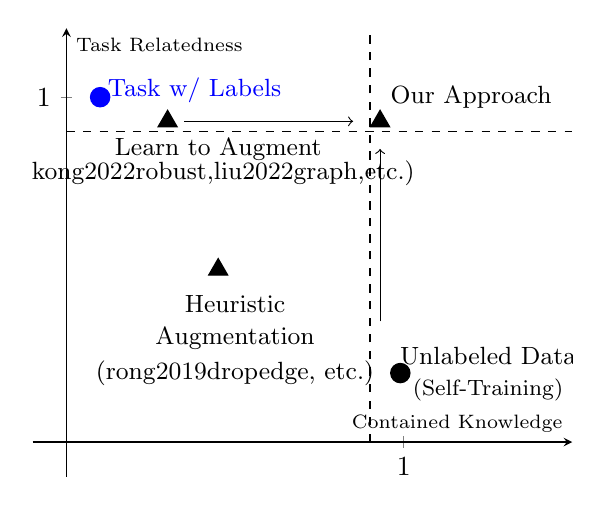
\begin{tikzpicture}
    \begin{axis}
    [
        legend pos= north east,
        axis lines = center,
        domain=-1:2,
        xlabel={\scriptsize Contained Knowledge},
        xmin=-0.1,
        xmax=1.5,
        xtick={0, 1},
        ylabel={\scriptsize Task Relatedness},
        ymin=-0.1,
        ytick={0, 1},
        ymax=1.2,
    ]
    % purple pentagon
    \addplot[only marks, color=black, mark=triangle*, mark size=4pt] coordinates { (0.93,0.93) };
    \node[] at (axis cs: 1.2, 1.0) {\textcolor{black}{\small Our Approach}};

    
    % magenta
    \addplot[only marks, color=black, mark=triangle*,mark size=4pt] coordinates {(0.3,0.93)};
    \node[] at (axis cs: 0.45,0.85) {\textcolor{black}{\small Learn to Augment}};
    \node[] at (axis cs: 0.45,0.78) {\small (\citeauthor{kong2022robust},\citeauthor{liu2022graph},etc.)};
    
    % cyan
    \addplot[only marks, color=black, mark=triangle*,mark size=4pt]
        coordinates {(0.45,0.5) };
    \node[] at (axis cs: 0.5,0.4) {\textcolor{black}{\small Heuristic}};
    \node[] at (axis cs: 0.5,0.3) {\textcolor{black}{\small Augmentation}};
    \node[] at (axis cs: 0.5,0.2) {\textcolor{black}{\small (\citeauthor{rong2019dropedge}, etc.)}};
    
    % red square
    \addplot[only marks, color=blue, mark=*, mark size=3.5pt]
        coordinates {(0.1,1)};
    \node[] at (axis cs: 0.38,1.02) {\textcolor{blue}{\small Task w/ Labels}};

    % color=blue
    \addplot[only marks, color=black, mark=*, mark size=3.5pt]
        coordinates {(0.99,0.2) };
    \node[] at (axis cs: 1.25,0.25) {\textcolor{black}{\small Unlabeled Data}};
    \node[] at (axis cs: 1.25,0.15) {\textcolor{black}{\footnotesize (Self-Training)}};
    
    \draw [dashed] (0.9,0) -- (0.9,1.2);
    \draw [dashed] (0,0.9) -- (1.5,0.9);
    \draw[->](axis cs: 0.35,0.93)--(axis cs: 0.85,0.93);
    \draw[->](axis cs: 0.93,0.35)--(axis cs: 0.93,0.85);
    % \draw[->](unlabeled)--(ours);
    \end{axis}
\end{tikzpicture}}
\end{wrapfigure} 
As presented in~\cref{fig: info relationship}, perturb edges, delete nodes and mask attributes~\citep{rong2019dropedge,trivedianalyzing} for graphs are some heuristic ways for data augmentation. The augmented knowledge from them is mainly controlled by human prior knowledge on the perturbations and it often fails to be close to the task, \ie, random perturbations hardly preserve labels for the augmented graphs. The learning to augment approaches learn from labeled graphs to perturb graph structures~\citep{luo2022automated}, to estimate graphons for different classes~\citep{han2022g}, or to split the latent space for augmentation~\citep{liu2022graph}. Although these approaches could preserve labels for the augmented graphs, they introduce less extra knowledge to improve the model prediction. In summary, graph data augmentation is effective in expanding knowledge for limited labels, but it makes no use of unlabeled graphs. Besides, the diversity and richness of the domain knowledge from augmented graphs are far from that contained in a large number of unlabeled graphs. To learn from unlabeled graphs, data-centric approaches like the self-training is assumed to be useful when the unlabeled and labeled data are from the same source. It is less studied when we have a single unified unlabeled source for different tasks.

\section{Additional Method Details}
\subsection{Upper bounding the mutual information}
In~\cref{eq:upper bound infonce}, we use a leave-one-out variant of InfoNCE ($\I_\text{bound}$) to derive the upper bound of mutual information. We summarize the derivation~\citep{poole2019variational} here.
\begin{equation}\label{eq:add derivation mi upper bound}
    \begin{split}
        \mathcal{I}_1(G^\prime;G) & = \mathbb{E}_{p (G, G^\prime)} \left[ \operatorname{log} \frac{p(G^\prime|G)}{p(G^\prime)} \right] \\
        & = \mathbb{E}_{p (G, G^\prime)} \left[ \operatorname{log} \frac{p(G^\prime|G) q(G^\prime)}{q(G^\prime) p(G^\prime)} \right] \\
        & = \mathbb{E}_{p (G, G^\prime)} \left[ \operatorname{log} \frac{p(G^\prime|G)}{q(G^\prime)} \right] - \operatorname{KL} (p(G^\prime) || q(G^\prime) ) \\
        & \leq \mathbb{E}_{p (G, G^\prime)} \left[ \operatorname{log} \frac{p(G^\prime|G)}{q(G^\prime)} \right]
        % \\ & = \mathbb{E}_{p(G)} \left[\operatorname{KL} (p(G^\prime| G) || q(G^\prime)) \right]
    \end{split}    
\end{equation}
The intractable upper bound is minimized when the variational approximation $q(G^\prime)$ matches the true marginal $p(G^\prime)$~\citep{poole2019variational}. 
For each $G_i$, its augmented output $G_i^\prime$, and $M-1$ negative examples with different labels, we could approximate $q(G_i^\prime) = \frac{1}{M-1} \sum_{j \neq i} p(G_i^\prime | G_j)$. So, we have
\begin{equation}
    \begin{split}
        \mathcal{I}_1(G^\prime_i, G_i) 
        & \leq  \operatorname{log} \frac{p(G_i^\prime| G_i)}{\frac{1}{K-1} \sum_{j=1, j\neq i}^M p(G_i^\prime | G_j)}
        \\ & = \operatorname{log} \frac{p(G_i^\prime| G_i)}{\sum_{j=1, j\neq i}^M p(G_i^\prime | G_j)} + \operatorname{log} (M-1)
        \\ & = \I_\text{bound} (G_i^\prime; G_i) + \text{constant}
    \end{split}
\end{equation}

\subsection{Extraction of Statistical Features on Graphs}\label{add:sec:raw feature}
For each molecule and polymer graph, we concatenate the following vectors or values for statistical feature extraction.
\begin{compactitem}
    \item the sum of the degree in the graph;
    \item the vector indicating the distribution of atom types;
    \item the vector containing the maximum, minimum and mean values of atoms weights in a molecule or polymer;
    \item the vector containing the maximum, minimum, and mean values of bond valence.
\end{compactitem}
For each protein-protein interaction ego-graph in the biology field, we use the sorted vector of node degree distribution in the graph as the statistical features.

\subsection{Technical Details for Graph Data Augmentation with Diffusion Model}\label{add:method:tech}

\paragraph{The Lookup Table from Atom Type to Node Embedding Space}
Given a graph $G$, we assume the node feature matrix on the graph is $\mathbf{X} \in \mathbb{R}^{n \times F_\text{n}}$, where $n$ is the number of nodes. The edge feature matrix is $\mathbf{E} \in \mathbb{R}^{m \times F_\text{e}}$, where $m$ is the number of edges. There are two ways for $G$ to represent the graph structure in practice. We can use either the dense adjacency matrix $\mathbf{A} \in \mathbb{R}^{n \times n}$ or sparse edge index $\mathbf{I}_e \in \mathbb{R}^{2 \times m}$. The diffusion model~\citep{jo2022score} on graphs prefers the former, which is more straightforward for graph generations. The prediction model prefers the latter because of its flexibility, and less computational cost and time. The transformation between two types of graph structure representation takes additional time. Particularly for molecular graphs, the node features used for generation (one-hot encoding of the atom type) and for prediction (see the official package of OGBG~\footnote{\url{https://github.com/snap-stanford/ogb/blob/master/ogb/utils/features.py}} for details) are different, which introduces extra time to process the graph data. For details, we (1) first need to extract discrete node attributes given the atom type and its neighborhoods; (2) we then need to use an embedding table to embed node attributes in a continuous embedding space; (3) the embedding features of nodes with their graph structure are inputted into the graph neural networks to get the latent representation for nodes. The reverse process for data augmentation in \method may need to repeatedly process graph data with steps (1) and (2). It introduces additional time. To address these technical problems, we build up a lookup table to directly map the atom type to the node embedding. We average the node attributes for the same type of node within the batch. We then use the continuous node attributes as weights to average the corresponding node embedding according to the table.

\paragraph{Instantiations of SDE on Graphs} According to~\citet{song2020score}, we use the Variance Exploding (VE) SDE for the diffusion process. Given the minimal noise $\sigma_{\min}$ and the maximal noise $\sigma_{\max}$, the VE SDE is:
\begin{equation}
\mathrm{d} G =\sigma_{\min }\left(\frac{\sigma_{\max }}{\sigma_{\min }}\right)^t \sqrt{2 \log \frac{\sigma_{\max }}{\sigma_{\min }}} \mathrm{d} \mathbf{w}, \quad t \in(0,1]
\end{equation}
The perturbation kernel is derived~\citep{song2020score} as:
\begin{equation}
p_{0 t}(G^{(t)} \mid G^{(0)})=\mathcal{N}\left(G^{(t)} ; G^{(0)}, \sigma_{\min }^2\left(\frac{\sigma_{\max }}{\sigma_{\min }}\right)^{2 t} \mathbf{I}\right), \quad t \in(0,1]
\end{equation}

On graphs, we follow~\citet{jo2022score} to separate the perturbation of adjacency matrix and node features:
\begin{equation}\label{eq:appendix:perturbation kernel}
    p_{0 t}(G^{(t)} \mid G^{(0)}) = p_{0 t}(\mathbf{A}^{(t)} \mid \mathbf{A}^{(0)}) p_{0 t}(\mathbf{X}^{(t)} \mid \mathbf{X}^{(0)}).
\end{equation}

\paragraph{The Sampling Algorithm in the Reverse Process for Graph Data Augmentation} We adapt the Predictor-Corrector (PC) samplers for the graph data augmentation in the reverse process. The algorithm is shown in~\cref{alg:diffusion augmentation}.
\begin{algorithm}[H]
   \caption{Diffusion-Based Graph Augmentation with PC Sampling}
   \small
   \label{alg:diffusion augmentation}
   \def\bfX{\mathbf{X}}
   \def\bfz{\mathbf{z}}
   \def\bfI{\mathbf{I}}
   \def\mclN{\mathcal{N}}
\begin{algorithmic}
    \STATE {\bfseries Input:} Graph $G$ with node feature $\mathbf{X}$ and adjacency matrix $\mathbf{A}$, the denoising function for node feature $\mathbf{s}_{\mathbf{X}}$ and adjacency matrix $\mathbf{s}_{\mathbf{A}}$, the fine-tune loss $\mathcal{L}_\textbf{aug}$, Lagevin MCMC step size $\beta$,  scaling coefficient $\epsilon_1$
    \STATE $\mathbf{A}^{(D)} \gets \mathbf{A} + \mathbf{z}_A $; \quad $\mathbf{z}_A \sim \mclN(\mathbf{0}, \bfI)$
    \STATE $\mathbf{X}^{(D)} \gets \mathbf{X} + \mathbf{z}_X $; \quad $\mathbf{z}_X \sim \mclN(\mathbf{0}, \bfI)$
    
   \FOR{$t=D-1$ {\bfseries to}  $0$}
    \STATE $\hat{G}_{(t+1)} \sim p_{0 t+1} ( \hat{G}_{(t+1)} |G^{(t+1)}) $ \COMMENT{inner-loop sampling with another PC sampler}
    
    \STATE $ \mathbf{S}_A = \frac{1}{2} \mathbf{s}_{\mathbf{A}}(G^{(t+1)}, t+1) - \frac{1}{2} 
    \alpha \nabla_{\mathbf{A}^{(t)}} \mathcal{L}_\textbf{aug}(\hat{G}_{(t+1)})$
    
    \STATE  $ \mathbf{S}_X = \frac{1}{2} \mathbf{s}_{\mathbf{X}}(G^{(t+1)}, t+1) - \frac{1}{2} 
    \alpha \nabla_{\mathbf{X}^{(t)}} \mathcal{L}_\textbf{aug}(\hat{G}_{(t+1)})$
    
    \STATE $\tilde{\mathbf{A}}^{(t)} \gets \mathbf{A}^{(t+1)} + g(t)^2 \mathbf{S}_A + g(t) \mathbf{z}_A $; \quad $\mathbf{z}_A \sim \mclN(\mathbf{0}, \bfI)$ \COMMENT{Predictor for adjacency matrix}
    \STATE $\tilde{\mathbf{X}}^{(t)} \gets \mathbf{X}^{(t+1)} +  g(t)^2 \mathbf{S}_X  + g(t) \mathbf{z}_X $; \quad $\mathbf{z}_X \sim \mclN(\mathbf{0}, \bfI)$ \COMMENT{Predictor for node features}
    \STATE $\mathbf{A}^{(t)} \gets \tilde{\mathbf{A}}^{(t)} + \frac{\beta}{2} \mathbf{S}_A + \epsilon_1 \sqrt{\beta} \mathbf{z}_A $; \quad $\mathbf{z}_A \sim \mclN(\mathbf{0}, \bfI)$ \COMMENT{Corrector for adjacency matrix}
    \STATE $\mathbf{X}^{(t)} \gets \tilde{\mathbf{X}}^{(t)} + \frac{\beta}{2} \mathbf{S}_X  + \epsilon_1 \sqrt{\beta} \mathbf{z}_X $; \quad $\mathbf{z}_X \sim \mclN(\mathbf{0}, \bfI)$ \COMMENT{Corrector for node features}
   \ENDFOR
   \STATE {return} $G^\prime  = ( \mathbf{A}^{(0)}, \mathbf{X}^{(0)})$
\end{algorithmic}
\end{algorithm}

\paragraph{The Algorithm of the Framework} The algorithm of the proposed data-centric knowledge transfer framework is presented in \cref{alg:dct stage 1} and \cref{alg:dct stage 2}. In detail, \cref{alg:dct stage 1} corresponds to \cref{sec:learning} and \cref{alg:dct stage 2} corresponds to \cref{sec:generating}.


\begin{minipage}{7cm}
\begin{algorithm}[H]
   \caption{The Data-Centric Knowledge Transfer Framework: Learning from Unlabeled Graphs}
   \label{alg:dct stage 1}
   \def\bfX{\mathbf{X}}
   \def\bfz{\mathbf{z}}
   \def\bfI{\mathbf{I}}
   \def\mclN{\mathcal{N}}
   \small
\begin{algorithmic}

    \STATE {\bfseries Input:} Given unlabeled graphs from the space $\mathcal{G}^{[U]}$, randomly initialized score models $\mathbf{s}_{\mathbf{X}}$ and $\mathbf{s}_{\mathbf{A}}$ for node feature and graph adjacency matrix, respectively, the total diffusion time step $T$.
    \WHILE{$\mathbf{s}_{\mathbf{X}}$ and $\mathbf{s}_{\mathbf{A}}$ not converged}
    \STATE Sample $G = (\mathbf{X}, \mathbf{A}) \in \mathcal{G}^{[U]}$
    \STATE Sample $t \in \operatorname{Uniform}({1, 2,\dots, T})$\
    \STATE Sample $\mathbf{z}_A \sim \mclN(\mathbf{0}, \bfI)$
    \STATE Sample $\mathbf{z}_X \sim \mclN(\mathbf{0}, \bfI)$
    \STATE Sample $\hat{G}$ with $t$, $\mathbf{z}_A$, $\mathbf{z}_X$ and~\cref{eq:appendix:perturbation kernel} 
    \STATE Optimize $\mathbf{s}_{\mathbf{A}}$ with the gradient: \\ \quad\quad   $\nabla \|\mathbf{z}_A - \mathbf{s}_{\mathbf{A}}(\hat{G}, t)  \|^2$
    \STATE Optimize $\mathbf{s}_{\mathbf{X}}$ with the gradient: \\ \quad\quad   $\nabla \|\mathbf{z}_X - \mathbf{s}_{\mathbf{X}}(\hat{G}, t)  \|^2$
    \ENDWHILE
\end{algorithmic}
\end{algorithm}
\end{minipage}
\hfil
\begin{minipage}{7.5cm}
\begin{algorithm}[H]
\vspace{0.02in}
   \caption{The Data-Centric Knowledge Transfer Framework: Generating Task-specific Labeled Graphs}
   \label{alg:dct stage 2}
   \def\bfX{\mathbf{X}}
   \def\bfz{\mathbf{z}}
   \def\bfI{\mathbf{I}}
   \def\mclN{\mathcal{N}}
   \small
\begin{algorithmic}
    \STATE {\bfseries Input:} Given task $k$ with the graph-label space ($\mathcal{G}, \mathcal{Y}$), a randomly initialized prediction model $f_\theta$, the well-trained score model  $\mathbf{s} = (\mathbf{s}_{\mathbf{X}}, \mathbf{s}_{\mathbf{A}})$, the training data set $\{G_i, y_i\}_i^{N_t}$, total training epoch $e$, the hyper-paramtere $n$
    \FOR{current epoch $e_i$ from 1 to $e$}
    \STATE Train $f_\theta$ on current training data $\{G_i, y_i\}_i^{N_t}$
    \IF{$e_i$ is divisible by the augmentation interval}
    \STATE Select $n$ graph-label pairs with the lowest training loss from $\{G_i, y_i\}_i^{N_t}$
    \STATE Get the augmented examples $\{G^\prime_i, y^\prime_i\}_i^{n}$ by~\cref{alg:diffusion augmentation} with the selected examples
    \STATE Update $\{G_i, y_i\}_i^{N_t}$ with $\{G^\prime_i, y^\prime_i\}_i^{n}$, \textit{e.g.,} add $\{G^\prime_i, y^\prime_i\}_i^{n}$ to $\{G_i, y_i\}_i^{N_t}$.
    \ENDIF
    \ENDFOR
\end{algorithmic}
\end{algorithm}
\end{minipage}

\section{Additional Experiments Set-ups}\label{sec: add exp setups}
We perform experiments on 15 datasets, including eight classification and seven regression tasks from chemistry, material science, and biology. We use Area under the ROC curve (AUC) for classification performance and mean absolute error (MAE) for regression.
\subsection{Molecule Classification and Regression Tasks}
Seven molecule classification and three molecule regression tasks are from open graph benchmark~\citep{hu2020open}. They were originally collected by MoleculeNet~\citep{wu2018moleculenet} and used to predict molecule properties. They include (1) inhibition to HIV virus replication in \hiv, (2) toxicological properties of 617 types in \toxcast, (3) toxicity measurements such as nuclear receptors and stress response in \toxt, (4) blood–brain barrier permeability in \bbbp, (5) inhibition to human $\beta$-secretase 1 in \bace, (6) FDA approval status or failed clinical trial in \clintox, (7) having drug side effects of 27 system organ classes in \sider, (8) predicting the property of lipophilicity in \lipo, (9) predicting the water solubility ($\log$ solubility in mols per litre) from chemical structures in \esol, (10) predicting the hydration free energy of molecules in water in \freesolv.
For all molecule datasets, we use the scaffold splitting procedure as the open graph benchmark adopted \citep{hu2020open}. It attempts to separate structurally different molecules into different subsets, which provides a more realistic estimate of model performance in experiments~\citep{wu2018moleculenet}.

\subsection{Polymer Regression Tasks}
Four polymer regression tasks include \glass, \melting, \thermal, and \oxygen. They are used to predict different polymer properties such as \emph{glass transition temperature} ($^\circ$C), \emph{melting temperature} ($^\circ$C), \emph{thermal conductivity} (W/mK) and \emph{oxygen permeability} (Barrer). \glass and \melting are collected from PolyInfo, which is the largest web-based polymer database \citep{otsuka2011polyinfo}. The \thermal dataset is from molecular dynamics simulation and is an extension from the dataset used in~\citep{ma2022machine}. The \oxygen dataset is created from the Membrane Society of Australasia portal,
consisting of a variety of gas permeability data \citep{thornton2012polymer}. Since a polymer is built from repeated units, researchers often use a single unit graph with polymerization points as polymer graphs to predict properties. Different from molecular graphs, two polymerization points are two special nodes (see ``$*$'' in \cref{fig:implementation}), indicating the polymerization of monomers \citep{cormack2004molecularly}. For all the polymer tasks, we randomly split by 60\%/10\%/30\% for training, validation, and test.

\subsection{Protein Classification Task}
An additional task is protein function prediction using protein-protein interaction graphs~\citep{hu2019strategies}. A node is a protein without attributes, an edge is a relation type between two proteins such as co-expression and co-occurrence. In our \method, we treat all the relations as the undirected edge without attributes.


\subsection{Baselines and Implementation}
When implementing \gin~\citep{xu2018powerful}, we tune its hyper-parameters for different tasks with an early stop on the validation set. We generally implement pre-training baselines following their own setting. For molecule and polymer property prediction and protein function prediction, the pre-trained \gin models with self-supervised tasks such as \edgepred, \attrmask, \contextpred in~\citep{hu2019strategies}, \infomax~\citep{velickovic2019deep} are available. So we directly use them. For other self-supervised methods, we implement their codes with default hyper-parameters. Following their settings, we use 2M ZINC15~\citep{sterling2015zinc} to pre-train \gin models for molecule and polymer property prediction. We use 306K unlabeled protein-protein interaction ego-networks~\citep{hu2019strategies} to pre-train the \gin for the downstream protein function property prediction. For self-training with real unlabeled graphs and \infograph~\citep{sun2019infograph}, we use 113K QM9~\citep{ramakrishnan2014quantum}. For self-training with generated unlabeled graphs, we train the diffusion model~\citep{jo2022score} on the real QM9 dataset and then produce the same number of generated unlabeled graphs. To train the diffusion model in our \method, we also use QM9~\citep{ramakrishnan2014quantum}.

\section{Additional Experiment Analysis}
\subsection{The Power of Diffusion Model to Learn from Unlabeled Graphs}
In~\cref{tab:ablation finetune}, when we replace the 133K QM9 with the 249K ZINC~\citep{jo2022score} to train the diffusion model, which nearly doubles the size of the unlabeled graphs and includes more atom types, we do not observe any additional improvement, and in some cases, even worse performance. It is possible because of the constraint of the current diffusion model's capacity to model the data distribution for a much larger number of more complex graphs. It encourages powerful generative models in the future, which could be directly used to benefit predictive models under the proposed framework.

\subsection{Chemical Validity of the Generated Graphs in Downstream Tasks}\label{add:sec:chemical_valid}
In \cref{fig:visual}, we show through some examples that concepts, such as certain chemical rules from the unlabeled graphs, are successfully transferred to downstream tasks. To further validate this point, we gathered 1,000 task-specific graphs generated in the intermediate steps on the tasks of \bace, \bbbp, \freesolv, and \oxygen. We then assessed the chemical validity of these graphs and observed that the validity is 92.8\%, 87.9\%, 97.4\%, and 62.1\%, respectively. Results show that transferring knowledge from pre-trained molecular data to target molecules yields relatively high chemical validity. However, the validity drops to 62\% when transferring knowledge from pre-trained molecular data to target polymer data. This finding indicates that the transferability of chemical rules becomes more challenging when the distribution gap between the pre-training data and downstream task data is larger.